\section{Referencia de la Clase Facturas\-List}
\label{classFacturasList}\index{FacturasList@{FacturasList}}
Administra el listado de facturas a clientes.  


{\tt \#include $<$facturaslist.h$>$}

Diagrama de colaboraci\'{o}n para Facturas\-List:\begin{figure}[H]
\begin{center}
\leavevmode
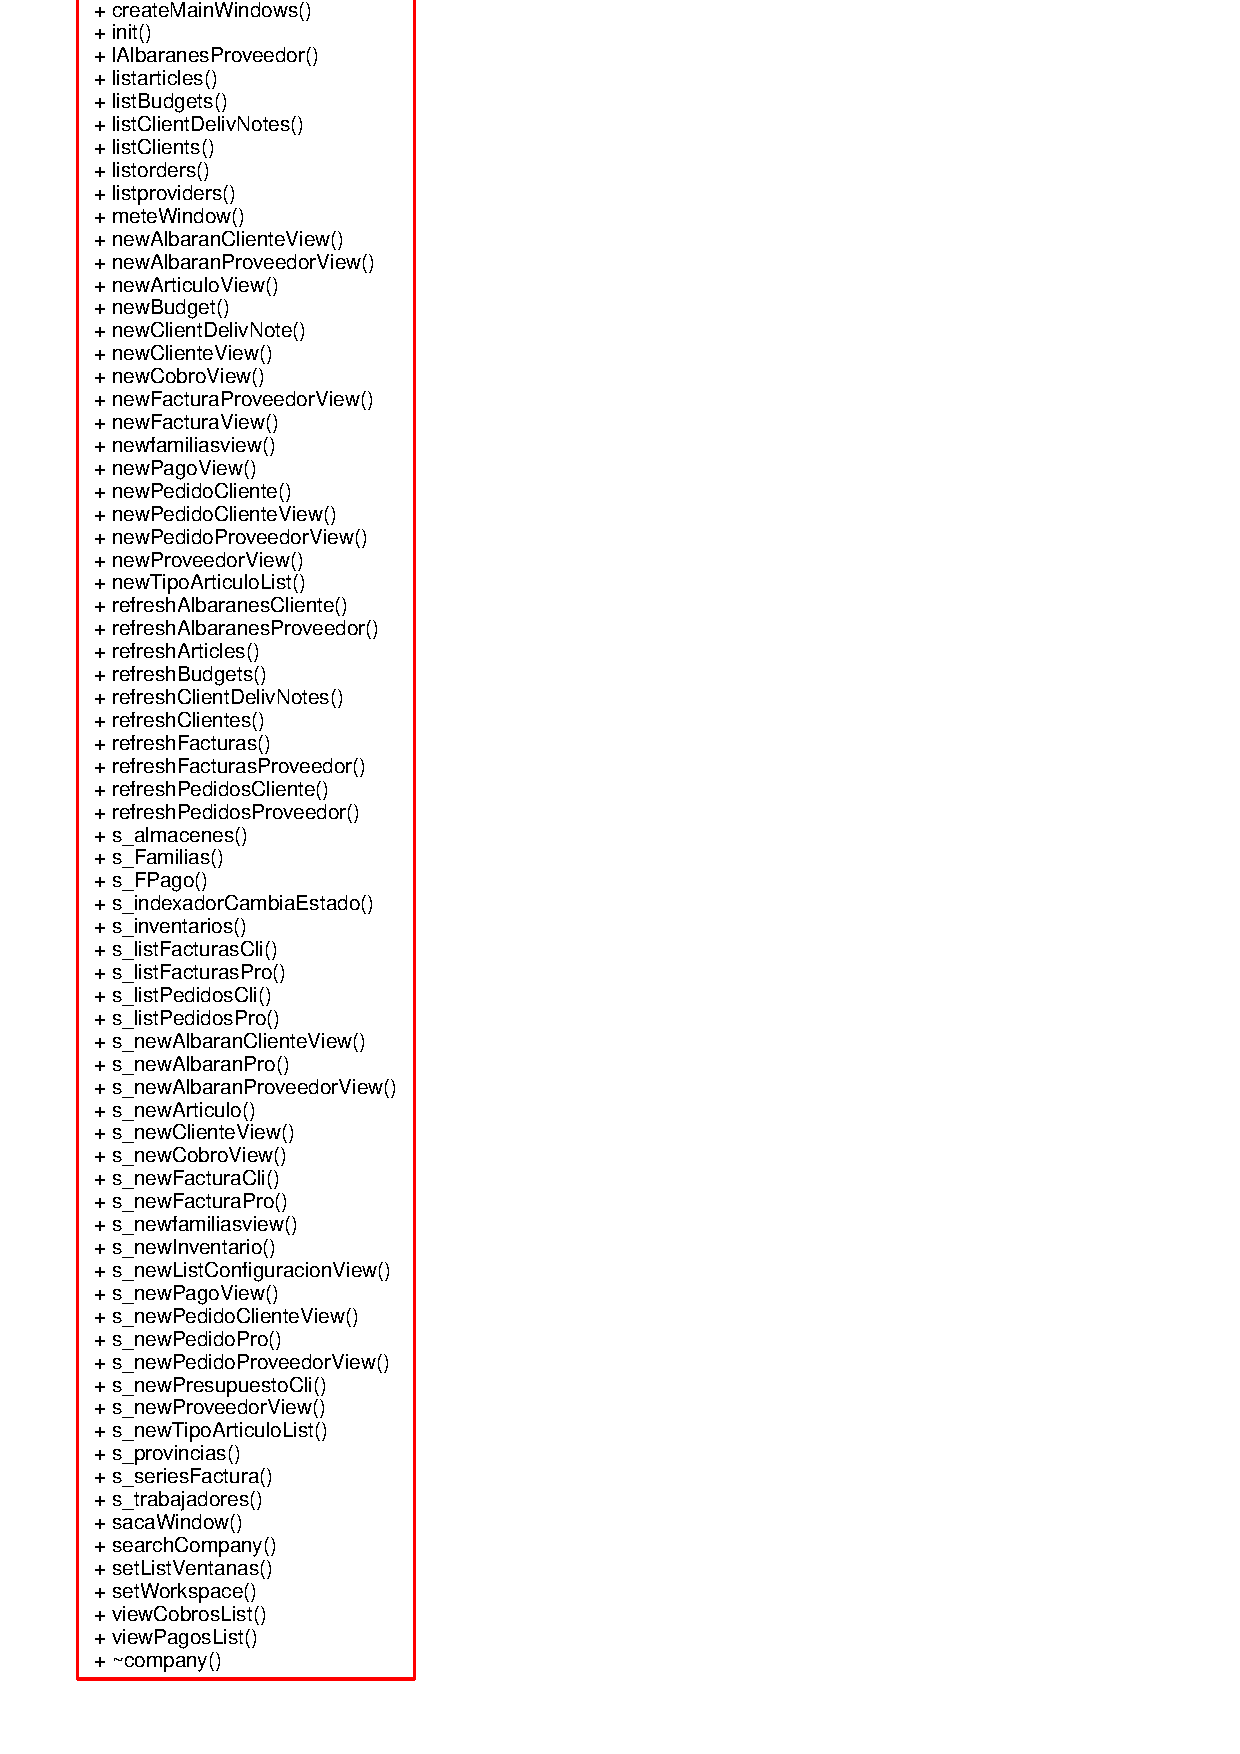
\includegraphics[width=119pt]{classFacturasList__coll__graph}
\end{center}
\end{figure}
\subsection*{Tipos p\'{u}blicos}
\begin{CompactItemize}
\item 
enum {\bf edmode} \{ {\bf Edit\-Mode} =  0, 
{\bf Select\-Mode} =  1
 \}
\end{CompactItemize}
\subsection*{Slots p\'{u}blicos}
\begin{CompactItemize}
\item 
virtual void {\bf on\_\-m\_\-filtro\_\-text\-Changed} (const QString \&text)\label{classFacturasList_i0}

\item 
virtual void {\bf on\_\-mui\_\-actualizar\_\-clicked} ()\label{classFacturasList_i1}

\item 
virtual void {\bf on\_\-mui\_\-borrar\_\-clicked} ()\label{classFacturasList_i2}

\item 
virtual void {\bf on\_\-mui\_\-configurar\_\-toggled} (bool checked)\label{classFacturasList_i3}

\item 
virtual void {\bf on\_\-mui\_\-crear\_\-clicked} ()\label{classFacturasList_i4}

\item 
virtual void {\bf on\_\-mui\_\-editar\_\-clicked} ()\label{classFacturasList_i5}

\item 
virtual void {\bf on\_\-mui\_\-imprimir\_\-clicked} ()\label{classFacturasList_i6}

\item 
void {\bf on\_\-mui\_\-list\_\-item\-Double\-Clicked} (QTable\-Widget\-Item $\ast$)\label{classFacturasList_i7}

\end{CompactItemize}
\subsection*{Se\~{n}ales}
\begin{CompactItemize}
\item 
void {\bf selected} (QString)\label{classFacturasList_l0}

\end{CompactItemize}
\subsection*{M\'{e}todos p\'{u}blicos}
\begin{CompactItemize}
\item 
void {\bf editar} (int)\label{classFacturasList_a0}

\item 
{\bf Facturas\-List} ({\bf company} $\ast$, QWidget $\ast$parent=0, Qt::WFlags flag=0, edmode editmodo=Edit\-Mode)\label{classFacturasList_a1}

\item 
{\bf Facturas\-List} (QWidget $\ast$parent=0, Qt::WFlags flag=0, edmode editmodo=Edit\-Mode)\label{classFacturasList_a2}

\item 
QString {\bf genera\-Filtro} ()
\item 
{\bf company} $\ast$ {\bf getcompany} ()\label{classFacturasList_a4}

\item 
void {\bf hide\-Busqueda} ()\label{classFacturasList_a5}

\item 
QString {\bf idfactura} ()\label{classFacturasList_a6}

\item 
void {\bf mete\-Window} (QString nom, QObject $\ast$obj)\label{classFacturasList_a7}

\item 
int {\bf modo} ()\label{classFacturasList_a8}

\item 
void {\bf modoedicion} ()\label{classFacturasList_a9}

\item 
void {\bf modoseleccion} ()\label{classFacturasList_a10}

\item 
void {\bf presenta} ()
\item 
void {\bf setcompany} ({\bf company} $\ast$comp)\label{classFacturasList_a12}

\item 
void {\bf setidarticulo} (QString val)\label{classFacturasList_a13}

\item 
void {\bf setidcliente} (QString val)\label{classFacturasList_a14}

\item 
void {\bf show\-Busqueda} ()\label{classFacturasList_a15}

\end{CompactItemize}


\subsection{Descripci\'{o}n detallada}
Administra el listado de facturas a clientes. 



\subsection{Documentaci\'{o}n de las funciones miembro}
\index{FacturasList@{Facturas\-List}!generaFiltro@{generaFiltro}}
\index{generaFiltro@{generaFiltro}!FacturasList@{Facturas\-List}}
\subsubsection{\setlength{\rightskip}{0pt plus 5cm}QString Facturas\-List::genera\-Filtro ()}\label{classFacturasList_a3}


Tratamiento de los filtros. \index{FacturasList@{Facturas\-List}!presenta@{presenta}}
\index{presenta@{presenta}!FacturasList@{Facturas\-List}}
\subsubsection{\setlength{\rightskip}{0pt plus 5cm}void Facturas\-List::presenta ()}\label{classFacturasList_a11}


Hacemos el calculo del total. 

La documentaci\'{o}n para esta clase fu\'{e} generada a partir de los siguientes archivos:\begin{CompactItemize}
\item 
facturaslist.h\item 
facturaslist.cpp\end{CompactItemize}
